\documentclass{article}
\usepackage{amsmath}
\usepackage{amssymb}
\usepackage{fancyhdr}
\usepackage[utf8]{inputenc}
\usepackage{tcolorbox}
\usepackage[left=1in, right=1in, top=1.5in, bottom=1in]{geometry}
\usepackage{tikz}
\usepackage{enumerate}
\usepackage{enumitem}
\usepackage{pgfplots}
\usepackage{ragged2e}
\usepackage{tabularx}
\usepackage{array}
\pagestyle{fancy}
\fancyhf{} % Clear all header and footer fields
\fancyhead[L]{Your Name} % Left header with name
\fancyhead[R]{September 18th 2025} % Right header with date
\renewcommand{\headrulewidth}{0.4pt} % Horizontal line below the header

\begin{document}

% Main title
\begin{center}
    \Large \textbf{Math 115E Activity 7} \\
    \vspace{0.2cm}
    \normalsize Chapter 3 Section 3 \\
    \normalsize Algebra of Functions
\end{center}
\hspace{4cm} \textbf{COMPLETE FOR 2 BONUS POINTS BY SEP 25TH}

\vspace{0.5cm}
\textbf{Continuation of Algebra of Functions}

\noindent
\begin{minipage}[c]{0.60\textwidth}
    \begin{enumerate}
        \vspace{0.5cm}
        \item Let $f(x)$ be the function given by the graph \\
              Let $g(x)$ be given as $g(x)=1-x-x^2$ \\
              Let $h(x)$ be the function given by the table
              \begin{center}
                \raggedright
                \begin{tabular}{|c||c|c|c|c|c|c|c|c|}
                    \hline
                    $x$ & -5 & -3 & -1 & 0 & 2 & 4 & 5 & 6 \\
                    \hline
                    $h(x)$ & -2 & -0.5 & 0.5 & 2 & 3 & 9 & 0 & 15 \\
                    \hline
                \end{tabular}
        \end{center}
              Find the following
              \begin{enumerate}
                \item Find $f(x)=2$
                \vspace{1.2cm}
                \item Find $g(f(3))$
                \vspace{1.2cm}
                \item Find $(f \cdot g)(2)$
                \vspace{1.2cm}
                \item Find $(f \cdot g)(0)$
                \vspace{1.2cm}
                \item Find $(h-f)(4)$
                \vspace{1.2cm}
                \item Find $(h \cdot f)(0)$
                \vspace{1.2cm}
                \item Find $h(g(2))$
                \vspace{1.2cm}
                \item Find $h(f(-1))$
                \vspace{1.2cm}
                
              \end{enumerate}
        \end{enumerate}
\end{minipage}%
\hfill
\begin{minipage}[c]{0.40\textwidth} % Minipage for the TikZ graph (increased width slightly for labels)
    \centering % Center the TikZ picture within its minipage
    \vspace{-10cm}
    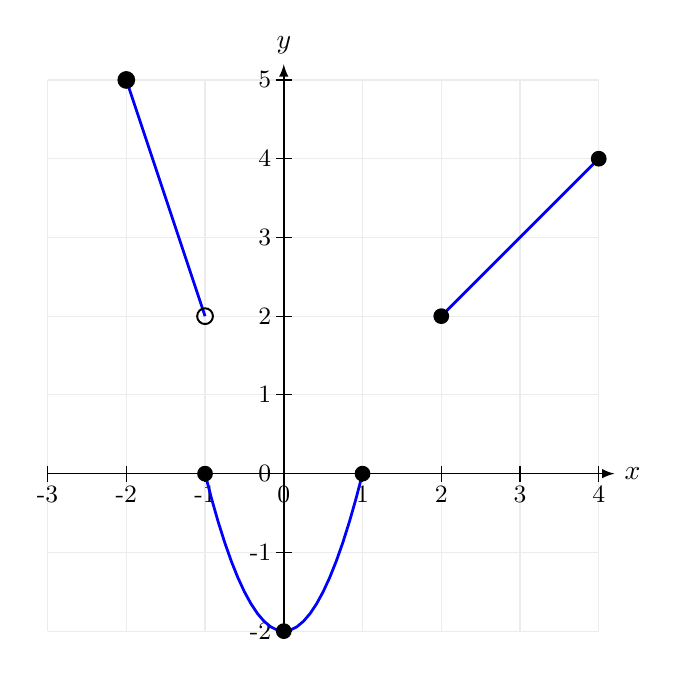
\begin{tikzpicture}[scale=1]
    \draw[gray!15,step=1cm] (-3,-2) grid (4,5);
    \draw[line width=0.2mm, -latex] (-3,0) -- (4.2,0) node[right] {$x$};
    \foreach \x in {-3,...,4} \draw (\x,.1)--(\x,-.1) node[below=1pt, font=\small] at (\x,0) {\x};
    \draw[line width=0.2mm,  -latex] (0,-2) -- (0,5.2) node[above] {$y$};
    \foreach \y in {-2,...,5} \draw (.1,\y)--(-.1,\y) node[left=1pt, font=\small] at (0,\y) {\y};

    % Slightly curved line from (-2,5) to (-1,2)
    \draw[blue, line width=1pt, smooth] plot coordinates {(-2, 5) (-1, 2)};
    \draw[fill=white, black, line width=0.25mm] (-2, 5) circle (0.1);
    \draw[black, line width=0.25mm] (-1, 2) circle (0.1);

    % Parabola from (-1,0) to (1,0) with vertex (0,-2)
    \draw[blue, line width=1pt] plot[domain=-1:1] (\x,{2*\x*\x - 2});
    \fill[black] (-1, 0) circle (0.1);
    \fill[black] (0, -2) circle (0.1);
    \fill[black] (1, 0) circle (0.1);

    % Straight line from (2,2) to (4,4)
    \draw[blue, line width=1pt] plot[domain=2:4] (\x, \x);
    \fill[black] (2, 2) circle (0.1);
    \fill[black] (4, 4) circle (0.1);

\end{tikzpicture}
    
    
\end{minipage}
\vspace{14cm}
\begin{enumerate}
    \setcounter{enumi}{1}
    \item Fill out the table using $g(x)=\frac{1}{3}x(x^2-10)+2$\\\\
    \begin{tabular}{|c|*{9}{|>{\centering\arraybackslash}p{0.75cm}}|}               
        \hline
        $x$     & -4 & -3 & -2 & -1 & 0  & 1  & 2  & 3 & 4 \\
        \hline
        $f(x)$  & -6 & -2 & 0  & -1 & 3  & 5  & -7 & 2 & 0 \\
        \hline
        $g(x)$  &    &    &    &    &    &    &    &   &   \\
        \hline
    \end{tabular}
    \\
    \begin{enumerate}
                \item Find $(f \cdot g)(3)$
                \vspace{1.2cm}
                \item Find $(f \cdot f)(3)$
                \vspace{1.2cm}
                \item Find $(g \cdot g)(-2)$
                \vspace{1.2cm}
                \item Find $g(f(3))$
                \vspace{1.2cm}
                \item Find $g(g(1))$
                \vspace{1.2cm}
                \item Find $g(f(1)-g(2))$
                \vspace{1.2cm}
                \item Find $f(g(1) + g(3))$
                \vspace{1.2cm}
                \item Find $g(g(3) \cdot f(4))$
                \vspace{1.2cm}
                \item Find $f(f(-2) \cdot f(2))$
                \vspace{1.2cm}
                \item Find $g(g(g(1)))$
                \vspace{1.2cm}
              \end{enumerate}
\end{enumerate}
\vspace{1cm}
\noindent

\end{document}